\section*{4.3 スマホアプリによるビーコンと実デバイス}
我々の利用するシステム「滞在ウォッチ」は実デバイスによるビーコンを利用した,ここではビーコンのアプリケーション化及びそれらのハイブリッド活用について記す.

 「滞在ウォッチ」は,先述の通りBLEビーコンを利用している.
 初めにBLEビーコンの仕様について解説する.
 BLEビーコンとはBLE規格のペリフェラル(Peripheral)動作を用いて,周囲にアドバタイズを行うデバイスとセントラル(Central)動作を用いて周囲をスキャンするデバイスによって構成される.
 ペリフェラル動作とは通信を受け付ける子機としての動作である.
 セントラル動作によってスキャンしたデバイスに反応しGATT(Generic attribute profile)内に保持したサービスやキャラクタリスティックのデータの送受信を行う.
 キャラクタリスティックとは,そのデバイスが保持するサービスやデータであり,今回の研究では個人識別符号として利用するUUIDが該当する.
UUID(Universally Unique Identifier)とは,オブジェクトを一位に識別するために重複がない前提で用いる128bitの数値である.
キャラクタリスティックのデータとしてこれをビーコンは保持している.


 実デバイスによるBLEビーコンは低コストでありサイズもコンパクトと携帯が用意である.しかしながら,メンバや管理者にとって利便性が低く結果として可用性が低くなる.
 可用性とは,メンバの在室情報が長期にわたり継続的に記録される能力と定義する.
 利便性における問題として,バッテリ切れによる問題,初期設定が複雑である問題が存在する.
まずはバッテリ切れによる問題である我々が利用しているビーコンはバッテリとしてCR2016を利用している.
このCR2016は一般的なコイン型リチウム電池であり,また実デバイスによるビーコンにバッテリ切れを通知する機能はない.
バッテリ残量の把握には,ビーコンメーカによる指定のアプリケーションを要し,実デバイスによるビーコン一台ごとに接続する必要がある.
また納入されたビーコンFCS1301はバッテリ切れによるデータ初期化が発生しない点を重視し購入したが,
我々がシステム運用をしている際にバッテリ切れが発生していない状態でも何故かUUIDが設定したものと
異なる数値に変更されてしまうケースが散見された.

他にも滞在ウォッチに特化したビーコン設定アプリを作ろうとした際,メーカにビーコン設定用アプリケーションに用いているライブラリについて相談したところ「メーカの専用アプリを利用してください」と期待通りの返答は得られなかった.
これらの状況から,実デバイスによるビーコンのみの運用では,メンバにとっての利便性が低下してしまい,それが原因としてシステムの可用性が低下してしまうと判断した.




\subsection*{4.3.1 BLEビーコンのアプリケーション化}
上記の問題のアプローチとしてメンバの利便性を向上させるため,スマホアプリによるビーコン動作を行った.

BLEビーコンの代替としてスマートフォンを利用可能にするとバッテリ交換の手間が削減される.
またスマートフォンユーザにとってスマートフォンはコミュニケーションツールとしての用途からバッテリ切れを配慮する傾向が強い.
実デバイスによるビーコンと比べてスマホビーコンはバッテリが維持されやすく利便性が向上すると考えた.
実デバイスによるビーコンには,バッテリ残量やバッテリ切れを通知するユーザインターフェースを持たない.
しかし,スマートフォンは液晶画面を持っており,スマートフォン自体のバッテリ残量やスマホアプリによるビーコンの動作状況など可視化が可能である.
そのためビーコンの動作状況を表示することでビーコン動作の停止に気が付きやすく,メンバによる再起動が行われた場合,可用性の向上が期待できる.
これらのメリットからスマートフォンアプリによるビーコン動作がユーザの利便性を向上させ,システムの可用性へつながると考えた.


\begin{figure}[tbh]
  \centering
  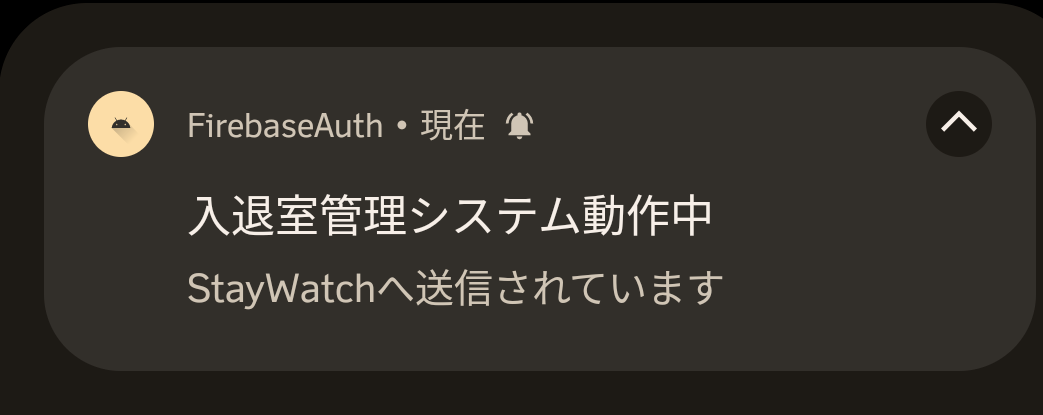
\includegraphics[width=12cm]{image/AppNofication.png}
  \caption{通知領域におけるビーコンの動作状況の表示}
  \label{multipleBPM}
\end{figure}


スマホビーコンは基本的にバックグラウンドに常在させる利用法を想定し実装した.
既存研究ではメンバに実デバイスによるビーコンを携帯させ,能動的な記録動作の必要がない.バックグラウンドに常在させる方式は実デバイスによるビーコンと同等の利便性がある.そのためバックグラウンドへの常在がアプリケーション化の前提である.
その点を踏まえて動作プラットフォームを選定した.
選定理由は技術調査をした際に,現状のiOSではフォアグラウンド動作はするもののバックグラウンド動作に制限がかかっており実デバイスによるビーコンと同等の利便性を担保することが困難であると判明したため,対応プラットフォームをAndroidのみにした.

実装に伴い,アプリケーションのプログラムはKotlinを用い,Bluetooth関連の実装においてはAltBeaconというライブラリを利用した.
また,ビーコン動作をする上で,Androidのプライバシ規則によって,バックグラウンド上でのユーザへの通知無しでの動作は禁止されている.
その点と,先述のスマートフォンが表示機能を持つ点を利用して 図           X        に示す通り   通知領域上でビーコン動作中は常時表示する仕様とした.
この仕様によってユーザが入退室のたびにアプリの起動を行う必要もなく,プライバシ規則を遵守した上で,実デバイスによるビーコンと同様の能動的な記録動作を要しない利便性を担保した.




ビーコンのアプリケーション化に伴い,管理者が実デバイスによるビーコンで行っていた登録作業をより簡略化した.
従来では管理者が新しいメンバが増えるたびに登録作業をおこない,Googleアカウント,名前,UUIDなどを登録し,
それに合わせて実デバイスによるビーコンへ割り当てられたUUIDを登録する作業を行っていた.
しかし先述の通り,Firabaseによるログインによって,スマホビーコン上で利用するUUIDをメンバに紐づいているメールアドレスでログインすることで,利用できるようにした.
% 手順は滞在WatchのWebページと同様である
\begin{figure}[tbh]
  \centering
  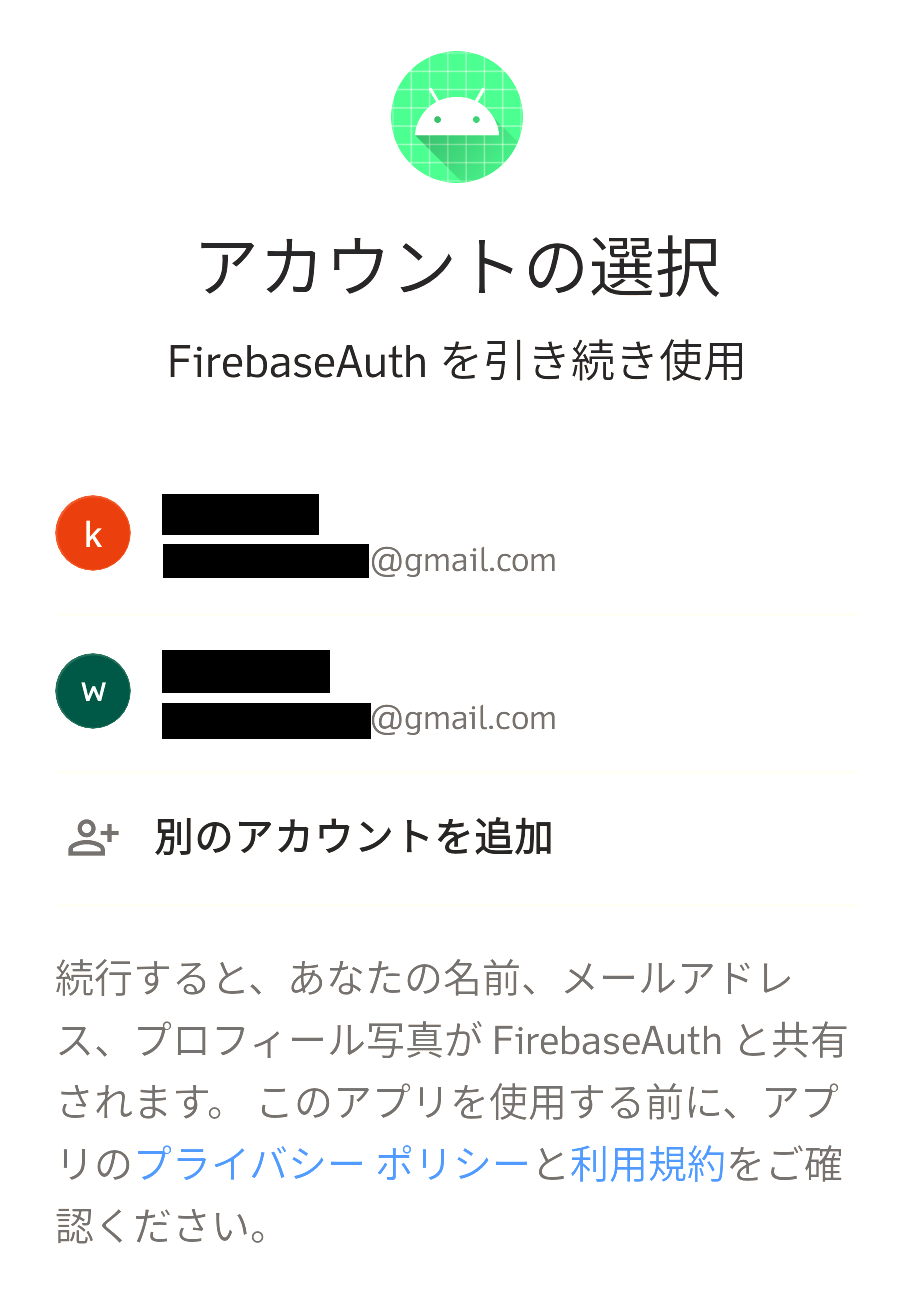
\includegraphics[width=9cm]{image/AppSignIn.png}
  \caption{アプリケーションのログイン画面}
  \label{multipleBPM}
\end{figure}


図    X    に示すサインインで管理者が登録したGoogleアカウントと一致する場合にログインを行う.その後APIからメンバの情報を受け取り,UUIDをアプリ内部に設定する.
以降はログイン時に受け取ったUUIDを用いたビーコン動作を行う.


% 画面の変更の写真を入れる
\begin{figure}[tbh]
  \centering
  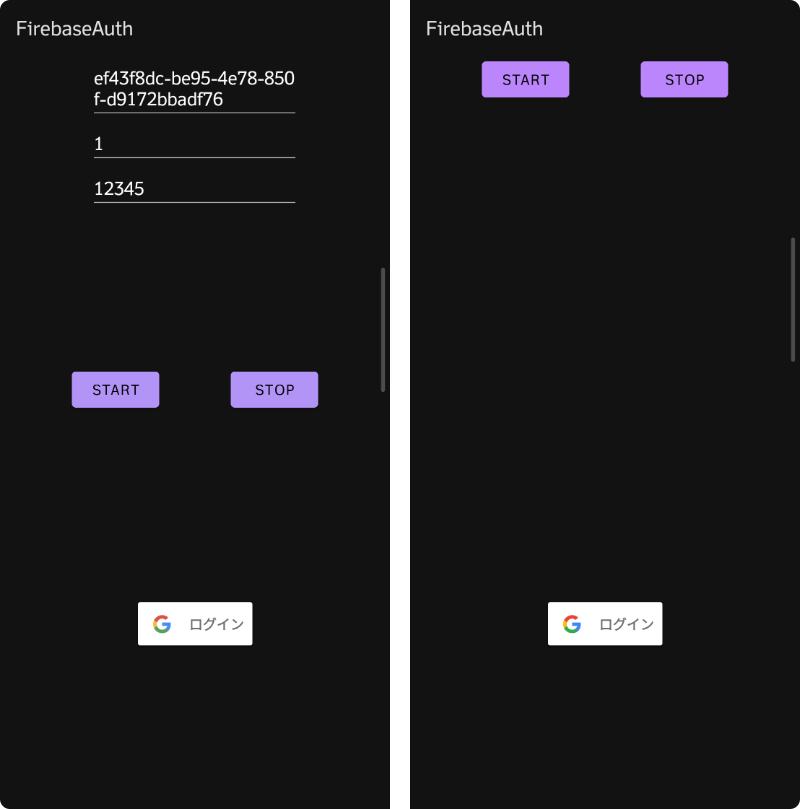
\includegraphics[width=9cm]{image/AppBeforeAfter.png}
  \caption{メンバ向けアプリケーションにおける操作の簡略化}
  \label{multipleBPM}
\end{figure}

また図  X   研究初期はユーザから利用しているUUID,major,minorを編集できる仕様にしていたが,複雑な操作がユーザの利便性の向上につながらないと考え取り消した.
% あと,実デバイスによるビーコンでは管理者がユーザ登録を行ったあと紐づけたビーコンに一台ずつ対応したUUIDを割り当てていたが,スマホビーコンならばウェブ上に登録されたユーザに紐づいたUUIDを持ってくる
% 4.2章が完成したときに整合性を取ろう!!!





\subsection*{4.3.2 スマホビーコンと実デバイスによるビーコンのハイブリッド活用}
スマホビーコンのみを利用する場合,様々な状況下でメンバの継続した利用が困難であるため,実デバイスによる
ビーコンと併用できるシステムとした.
長期にわたり継続的に利用するメンバにとっては,実デバイスによるビーコンは先述の通りバッテリ交換の手間がある.
スマホビーコンはそのようなメンバにとっては,バッテリ交換の手間がないため有用である.
しかしスマートフォンを携帯していないメンバ,スマホビーコンの利用に伴うバッテリ消費が気になるメンバなども想定される.
これらの問題は実デバイスによるビーコンとスマホビーコンのハイブリッド化に
よって解決できる.スマホビーコンで利用する UUID を
実デバイスによるビーコンで利用する UUID と同じ値に設定し同じメンバの在室情報を記録している.
この方法は表      X        に示す通りスマホビーコンか実デバイスによるビーコンの少なくとも片方を携帯していれば記録できるため
継続的にデータを記録する観点から見ても有用である.


% レジュメの内容にシチュエーションを加える 例 一時的な来訪者

% \begin{table}[tbh]
%   \centering
%   \caption{各ビーコンのみとハイブリッド対応時の比較}
%   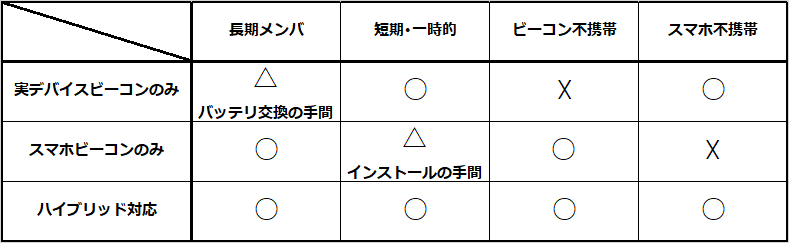
\includegraphics[width=15cm]{image/table.png}
%   \label{multipleBPM}
% \end{table}

\begin{table}[tbh]
  \caption{各ビーコンのみ対応時とハイブリッド対応時の比較}
      \begin{tabular}{|c|c|c|c|c|}
              \hline
               &  長期  メンバ  &  短期・一時的 &  スマホ不携帯  & ビーコン不携帯 \\ \hline
               \begin{tabular}[c]{@{}c@{}}実デバイス\\ ビーコンのみ\\\end{tabular}& \begin{tabular}[c]{@{}c@{}}\\△\\ バッテリ交換の手間\end{tabular} & ○ & X & ○ \\ \hline
               \begin{tabular}[c]{@{}c@{}}スマホ\\ ビーコンのみ\\\end{tabular}& ○ & \begin{tabular}[c]{@{}c@{}}\\△\\ インストールの手間\end{tabular} & ○ & X \\ \hline
               \begin{tabular}[c]{@{}c@{}}ハイブリッド\\ 対応\\\end{tabular} & \begin{tabular}[c]{@{}c@{}}\\○\\\\\end{tabular} & ○ & ○ & ○ \\ \hline
              \end{tabular}
  \label{multipleBPM}
\end{table}

